% LaTeX .tex example for the proceedings of
% COBEM 2017 - 24th International Congress of Mechanical Engineering
% December, 3-8, 2017, Curitiba, PR, Brazil
%
% Based on the template of the proceedings of COBEM2015 
% MODELO COBEM 2017

\documentclass[draft]{svjour3}

\usepackage{engsymbols}
\usepackage{magref}
\usepackage[utf8]{inputenc}
\usepackage{nicefrac}

\newcommand{\bmax}{\ensuremath{{B}\ped{max}}}
\newcommand{\bmin}{\ensuremath{{B}\ped{min}}}

\usepackage{mathptmx}
\journalname{Journal of the Brazilian Society of Mechanical Sciences and Engineering}

\usepackage{graphicx}
\usepackage{subfig}
\usepackage{xcolor}
\usepackage{nomencl}
\usepackage{hyperref}

\begin{document}

\title{Performance of Magnetic Refrigerators Operating with Different Magnetic Profiles}

\author{
Fábio P. Fortkamp \and
Gusttav B. Lang \and
Jaime A. Lozano \and
Jader R. Barbosa Jr.
}


\institute{
Fábio P. Fortkamp 
\at
POLO --- Research Laboratories for Emerging Technologies in Cooling and Thermophysics, Department of Mechanical Engineering, Federal University of Santa Catarina, Florianópolis, SC, 88040-900, Brazil, \email{fabio@polo.ufsc.br}
\and
Gusttav B. Lang \and
Jaime A. Lozano \and
Jader R. Barbosa Jr. \at POLO --- Research Laboratories for Emerging Technologies in Cooling and Thermophysics, Department of Mechanical Engineering, Federal University of Santa Catarina, Florianópolis, SC, 88040-900, Brazil}


\date{}


\maketitle

\begin{abstract}


\keywords{ magnetic refrigeration \and active magnetic regenerator \and numerical modeling \and magnetocaloric effect}
\end{abstract}

\section{Introduction}
\label{sec:introduction}

Mechanical vapor compression has been the dominant cooling technology for the past century \cite{bib:nik} but, despite its dominance, it still faces an increasing number of challenges related to the its environmental footprint. The large entropy generation associated with vapor compression processes makes this techonology constrained by low exergy efficiencies, in particular for compact systems \cite{KITANOVSKI2015288}. In addition, the phase-out of refrigerants \textcolor{black}{with} ozone depleting \textcolor{black}{and global warming potentials has} introduced the use of flammable substances, with their own set of risks for consumer applications \cite{bib:iir-flammable} and technologial challenges \cite{bib:lionte18-adapt}.

The term \emph{caloric cooling} is \textcolor{black}{generally} applied to alternative cooling techonologies in which the cooling effect is generated by the response of a solid material to a physical \textcolor{black}{stimulus}. The absence of hazardous gases, compressors \textcolor{black}{and throttling devices} makes these technologies potentially more efficient, \textcolor{black}{scalable}, silent and environmentally friendly. Magnetic refrigeration (MR) is the most advanced of all caloric technologies \cite{KITANOVSKI2015288}; in particular, with the classes of magnetic refrigerants currently available, magnetocaloric refrigeration seems promising for applications in small temperature span (around \SI{20}{\kelvin}), such as winecoolers \textcolor{black}{and air conditioners} \cite{KITANOVSKI2015288}.

\nomenclature[vm]{MR}{Magnetic (or Magnetocaloric) Refrigeration}

In magnetic refrigeration, a \emph{magnetocaloric material} (MCM) \textcolor{black}{is subjected to a cyclical change of the applied} magnetic field, and its temperature \textcolor{black}{changes as a result} of the \emph{magnetocaloric effect} (MCE). The magnitude of the MCE  \textcolor{black}{depends} on  parameters \textcolor{black}{related to} characteristics of the material, magnetic field variation and temperature, and its maximal at the transition Curie temperature of the material. For a thorough introduction to the magnetocaloric effect and magnetocaloric materials, the reader is referred to \cite{bib:smith-magneto}.

\nomenclature[vm]{MCM}{Magnetocaloric Material}

For operating conditions typical of a low-temperature span magnetic refrigerator, the MCE is typically \textcolor{black}{on} the order of \num{2}-\SI{5}{\kelvin}. \textcolor{black}{T}o amplify this \textcolor{black}{temperature change}, heat regeneration is usually employed \cite{bib:kitanovski}. Active magnetic regenerators (AMR) are thermal devices where the magnetocaloric material constitutes a solid matrix through which flows an aqueous heat transfer fluid, and is cyclically magnetized and demagnetized to activate the magnetocaloric effect.  \textcolor{black}{A regenerator is essentially a cascade of infinitesimal ``layers'' of MCM that are activated simultaneously} to build up a temperature profile \textcolor{black}{along its length}. These layers can be made of the same material, yielding an homogeneous regenerator; however, given the  dependence  of the MCE with temperature, it is an interesting strategy to build \emph{multilayer} regenerators, where each layer is composed of a different material \textcolor{black}{that} will work around its \textcolor{black}{own} Curie temperature, maximizing the magnetocaloric effect of each portion.

\nomenclature[vm]{AMR}{Active Magnetic Regenerator}

The five main subsystems in an AMR-based magnetic refrigerator can be identified as follows \cite{bib:jaime,bib:trevizoli16_pump}:

\begin{enumerate}
\item magnetic circuit; \label{item:1}
\item active magnetic regenerator; \label{item:2}
\item flow management system; \label{item:3}
\item control system; \label{item:4}
\item transmission system; \label{item:5}
\item heat exchangers and cabinet. \label{item:6a}
\end{enumerate}

The magnetic circuit generates oscillating magnetic fields that activate the MCE \textcolor{black}{in} the active magnetic regenerators. As previously explained, the regenerators are composed of magnetocaloric porous media, and the flow management system provides the alternating fluid flow through the beds. The control system \textcolor{black}{serves} the purpose of synchronizing the fluid flow regime with the magnetic field variations. Finally, the heat exchangers are responsible for transferring the cooling effect from the AMR to the refrigerated cabinet and the rejected heat to the surroundings. 

Magnetic refrigerators can operate according to different thermodynamic cycles, but the stages are roughly as follows. The magnetic circuit magnetizes the MCM, increasing its temperature due to the MCE. During the so-called \emph{cold blow}, cold fluid from the cold source flows through the warm bed and absorbs its energy, releasing it to the external heat exchanger. On the return of the fluid, the solid is demagnetized and cooled down, and in the \emph{hot blow} the fluid relases energy to the bed, decreasing its temperature so it can absorb the thermal load at the cold source. The cycle then repeats; different cycles can be configured by different durations and synchronization steps between these two \emph{characteristic waveforms}:

\begin{enumerate}
\item The \emph{magnetic profile}, which describes the oscillating magnetic field over one regenerator;
\item The \emph{fluid flow profile}, which describes the time-variation of flow rate through one bed.
\end{enumerate}

Among the challenges cited in the literature for further improvement of magnetic refrigerators, two can be highlighted \cite{bib:eriksen16_activ}:

\begin{enumerate}
\item Better use of AMR and magnetic circuit models during the design process, to identify optimal geometric and operating parameter;
\item Better study of losses that are present in a magnetic cooling device.
\end{enumerate}

\textcolor{black}{In} other words, these challenges arise due to \emph{interactions} between different subsystems \textcolor{black}of a magnetic refrigerator. In these context, the focus on the aforementioned waveforms is a suitable approach for optimizing the performance of magnetic refrigerators, as these profiles represent interactions between systems. As it will be seen, mathematical models for AMRs take these waveforms as input, and they are generated by models for other components.

Fluid flow profiles are more easily investigated with experimental methods, since they can be altered with modifications in the fluid flow system. In particular, the \emph{duration} of blows have been extensively investigated \cite{bib:teyber17_exper,bib:nakashima18-influen-exp,FORTKAMP2018}, and the literature shows that the cooling capacity of magnetic refrigerators can be increased by focusing fluid flows during periods where the magnetic field is at its extrema values.

In this work, we focus on magnetic profiles, which are less studied in the literature. The studied waveforms are depicted in \autoref{fig:profiles}, identified by the transitions between states. The instantaneous profile represents step-like changes between high and low levels of the magnetic field, while the ramp profile has linear variations between these states. The rectified cosine profile is a common waveform found in the literature that has a continuous variation of the applied magnetic field.

\begin{figure}[!ht]
  \centering
  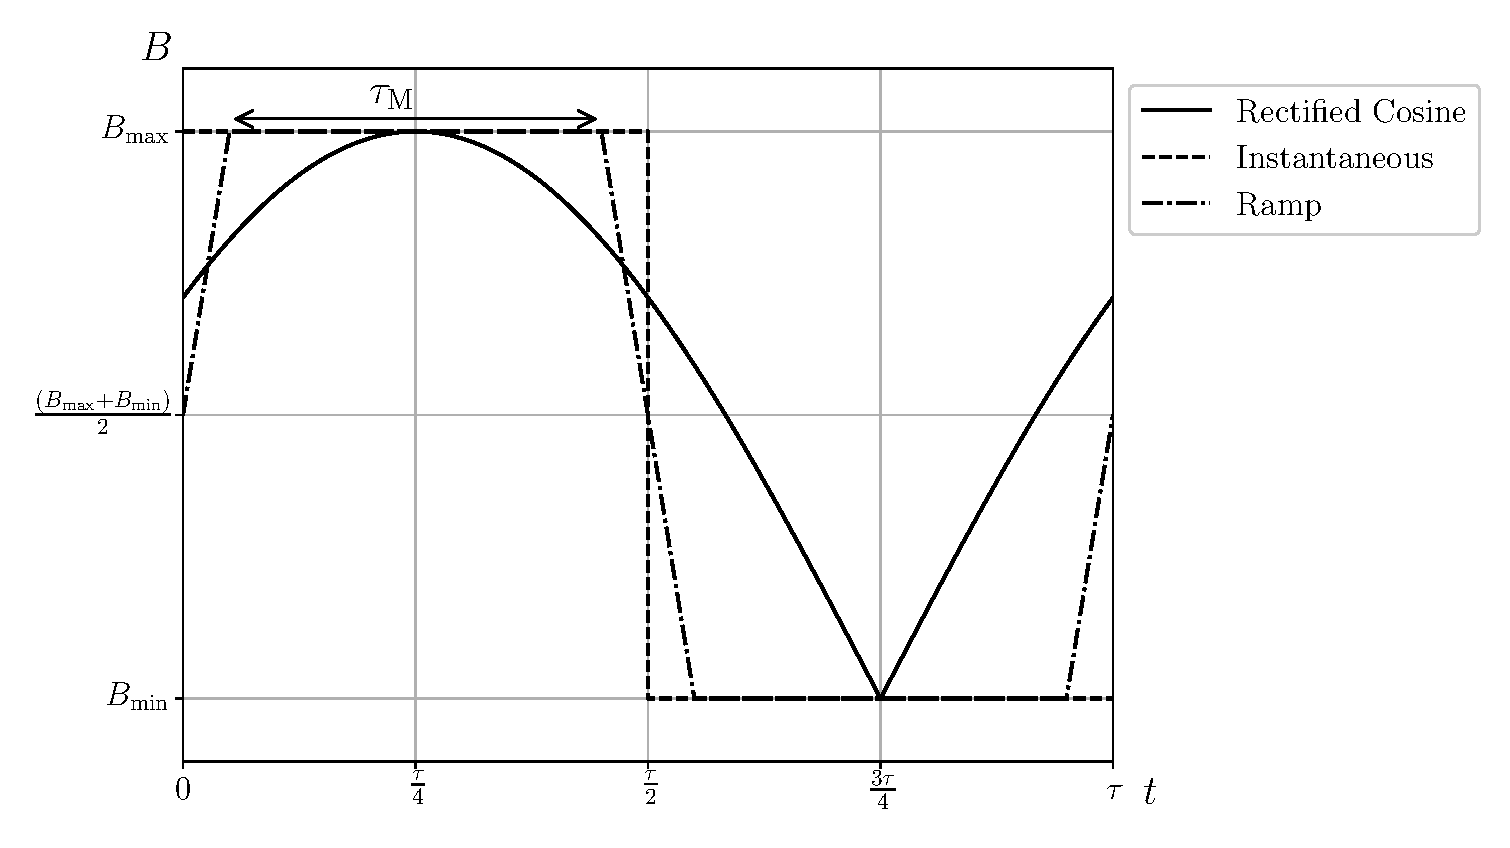
\includegraphics[width=8cm]{profiles_all}
  \caption{Magnetic profiles studied in this paper}
  \label{fig:profiles}
\end{figure}

The instantaneous magnetic profile is characteristic of the Brayton AMR cycle, where the magnetization and demagnetization steps must be done adiabatically, as shown in \autoref{fig:brayton}; compared to other common cycles such as the Ericsson, the Brayton cycle results in the highest cooling capacities for the same operating  parameters \cite{bib:kitanovski}, at the expense of lower coefficient of performance.


\begin{figure}[!ht]
  \centering
  
  \caption{Brayton AMR cycle}
  \label{fig:brayton}
\end{figure}

 In practice, the ramp profile is a more feasible realization with finite transition times, and its synchronization with the fluid flow profile can yield different performance levels \cite{TUSEK20111507}. In particular, the plateaus of magnetic field should be centered with the blow durations \cite{bib:bjoerk11_amr}.
\autoref{fig:sync} shows the syncronization schema between the magnetic and fluid flow profiles, showing the ramp magnetic profile as an example. 

\begin{figure}[!ht]
  \centering
  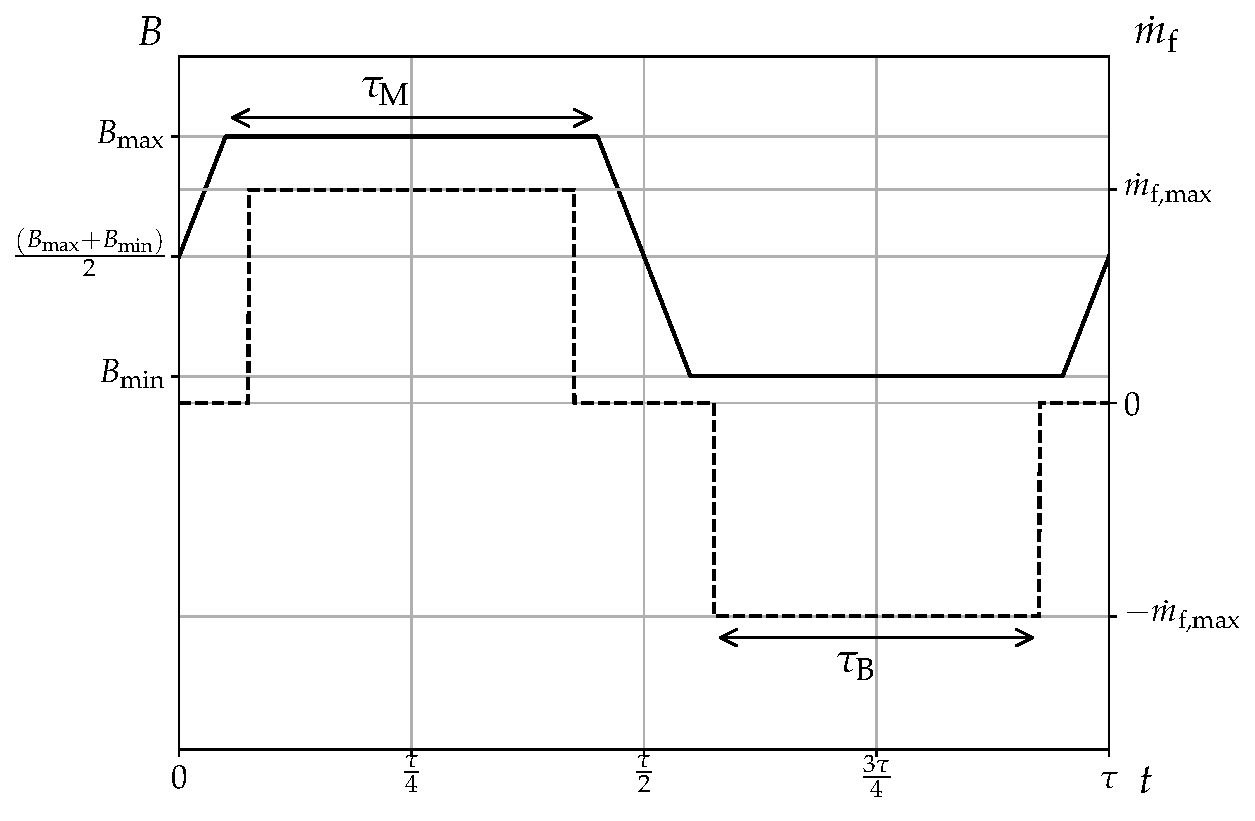
\includegraphics[width=8cm]{profiles_rm_and_flow_instantaneous}
  \caption{Ramp magnetic profile (solid lines) and instantaneous fluid flow profile (dashed lines)}
  \label{fig:sync}
\end{figure}

This paper uses the AMR model developed by \cite{bib:trevizoli16_perfor_model}, and the same authors had studied magnetic profiles waveforms in an earlier work \cite{bib:asme-mce}. However, their amplitudes was not varied, nor were they investigated with different geometries.

The present works combines the gaps from the above cited papers in investigating the performance of a magnetic refrigerator under different magnetic profile waveforms. These waveforms are mathematically modeled, and the cooling capacity and coefficient of performance are calculated based on the profiles parameters, while also investigated how the AMR geometry affect the performance in combinations with the magnetic profile. The fluid flow profile is assumed fixed in shape, although its parameters are also variied. The emulate constraints on an operating point of actual magnetic refrigeration devices, the temperature span is set fixed, and hence few comments are made on second-law efficiency.



\section{NUMERICAL SIMULATIONS}
\label{sec:numer-simul}

Simulations were performed using a one-dimensional AMR mathematical model \cite{bib:asme-mce,bib:trevizoli16_perfor_model}. The simulated magnetic refrigerators are composed of multiple prismatic regenerators filled with gadolinium (Gd) spheres as the magnetocaloric solid matrix, with the parameters shown in Table~\ref{tab:params}. The fluid is a mixture of water and ethylene glycol, in the proportion of \SI{80}{\percent}-\SI{20}{\percent} in volume.

\begin{table}[!ht]
  \centering
  \caption{Geometric and operation parameters for the simulated AMR devices}
  \begin{tabular}{c|c}
\hline
    \textbf{Parameter}&\textbf{Value}\\
\hline
Regenerator height & \SI{20}{\mm}\\
Regenerator width & \SI{25}{\mm}\\
Regenerator length & \SI{100}{\mm}\\
Number of regenerators & \num{11} \\
Particle diameter & \SI{0.5}{\mm}\\
Hot source temperature & \SI{298}{\kelvin}\\
Cold source temperature & \SI{278}{\kelvin}\\
\hline
  \end{tabular}
  \label{tab:params}
\end{table}

The AMR model solves mass and energy conservation equations for the solid and the fluid domains in an active magnetic regenerator. In this work, regenerators were assumed to be adiabatic to the environment. All beds experience the same flow and magnetic profiles, as detailed in the following sections.

\subsection{Flow profile}
\label{sec:flow-profile}


The flow profile through a given bed, i.e. the mass flow rate as a function of time $\rate{m}\ped{f} (t)$, is assumed to be a square wave as that shown in Fig.~\ref{fig:mprofile}. The cold blow has a duration of $\tau\ped{CB}$ and the  hot blow a duration of $\tau\ped{HB}$, while the period of one AMR cycle is $\tau$. Limiting the blow times during each half-cycle to periods where the magnetic field is at its maximum and minimum can result in increased performance \cite{bib:nakashima17_avaliac}. In this work, the blows are supposed to be in balance, thus, $\tau\ped{CB} = \tau\ped{HB}$. An important parameter regarding the flow profiles can be defined, which is the blow fraction, $F\ped{B}$:

\begin{equation}
  \label{eq:1}
  F\ped{B} = \frac{\tau\ped{CB} + \tau\ped{HB}}{\tau}
\end{equation}

\begin{figure}[!ht]
  \centering
%  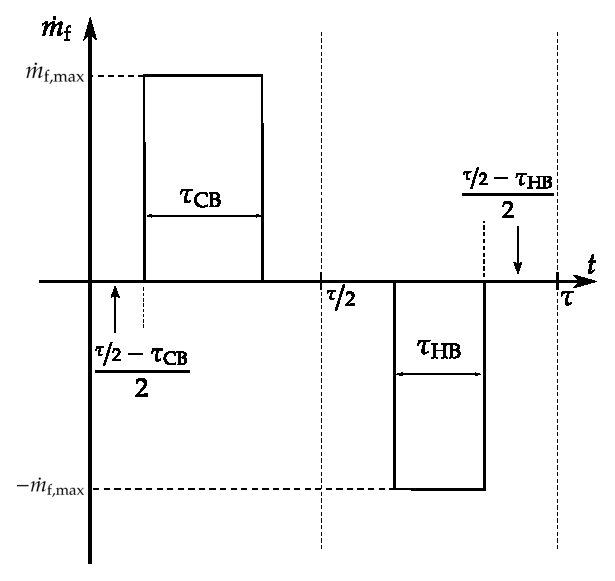
\includegraphics[width=7cm]{mprofile}
  \caption{Instantaneous flow profile used in the numerical simulations. "Positive" mass flow rate indicates flow in the direction from the cold to the hot source, and negative values represent the opposite direction. }
  \label{fig:mprofile}
\end{figure}

\subsection{Magnetic profile}
\label{sec:magnetic-profile}

The AMR mathematical model takes the magnetic profile as an input, and the profiles represented in Fig.~\ref{fig:cycles} were tested with different parameters. The mathematical definitions for the magnetic profiles over a cycle of period $\tau$ are as follows; the instantaneous profile (represented by the index ``I'') and the rectified cosine profile (represented by ``RC'') are defined solely in terms of the extrema values $\bmax$ and $\bmin$:

\begin{equation}
\average{B}\ped{I}(t)=
\begin{cases}
\average{B}\ped{max}, & 0 \le t < \nicefrac{\tau}{2} \\
\average{B}\ped{min}, & \nicefrac{\tau}{2} \le t < \tau\\
\end{cases}
\label{eq:4}
\end{equation}

\begin{equation}
\average{B}\ped{RC}(t) = \bmin + \left(\bmax - \bmin\right)  \left\lvert \cos\left( \frac{\pi}{\tau} \left( t - \frac{\tau}{4}\right)\right) \right\rvert
\label{eq:5}
\end{equation}


In this work, the average values of the magnetic field during each half-AMR cycle are considered for comparison between profiles. The average magnetic profile during the hot cycle ($0 \le t < \nicefrac{\tau}{2}$) is denoted $B\ped{h}$ and the average during the cold cycle  ($ \nicefrac{\tau}{2} \le t < \tau$) is denoted $B\ped{l}$.

\subsection{AMR operating parameters}
\label{sec:amr-oper-param}


Different numerical simulations were carried with different operating parameters such as: AMR cycle frequency ($f$), blow fraction ($F\ped{B}$) and utilization ($\Phi$) which is defined as:

\begin{equation}
\Phi = \frac{\rate{m}\ped{f,max}F\ped{B}\frac{\tau}{2}c_{p,\mathrm{f}}}{m\ped{s} c\ped{s}}
\label{eq:2}
\end{equation}

\noindent where $c_{p,\mathrm{f}}$ is the constant-pressure specific heat for the fluid, and $m\ped{s}$ and $c\ped{s}$ are the mass and specific heat of the solid phase in one bed. 

\section{RESULTS AND DISCUSSIONS}
\label{sec:results-discussions}

\subsection{Comparison of the instantaneous and rectified cosine profiles}
\label{sec:comp-inst-cosine}

When comparing the magnetic profiles, the average magnetic field during the hot cycle is the same; this implies in a higher peak for the rectified cosine. For the cold cycle, there are two possible comparison methods:

\begin{enumerate}
\item The minimum values for both profiles is the same;
\item The average value for both profiles during the cold cycle is the same.
\end{enumerate}

As a reference, in all simulations  the minimum value for the rectified cosine was fixed at $\average{B}\ped{min,RC} = \SI{0.1}{\tesla}$. For the first comparison, the minimum value for the instantaneous value was kept at the same level ($\average{B}\ped{min,I} =  \average{B}\ped{min,RC}$), hence, the average low value for the RC profile was higher ($B\ped{l,RC} > B\ped{l,I}$). Although this does not seem a fair comparison, in practice it is feasible to generate a profile with a constant low-valued plateau for the magnetic field \cite{bib:insinga16_optim,bib:benedict16_desig}. For the other comparison method, the low level of the instantaneous profile was increased ($\average{B}\ped{min,I} >  \average{B}\ped{min,RC}$) to keep the average the same ($B\ped{l,RC} = B\ped{l,I}$). In addition, simulations were ran for various values of blow fraction and the optimal cases were selected; the rectified cosine profile can benefit from a smaller blow fraction because this can concentrate the flow during the periods of very high or low fields. In this section, all results show the resulting optimal case of the blow fraction for each profile (for the values tested): fluid flowing during the entire period for the instantaneous profile, and only during \SI{60}{\percent} of the period for the cosine profile.


Figure~\ref{fig:cos_ins} shows the cooling capacity attained by the device at a frequency of \SI{1}{\hertz} and different utilizations, for both comparison methods.  The horizontal axis shows the average value during the high field region. Notice how the results are conflicting; for Fig.~\ref{fig:comp_min}, the instantaneous profile almost always yields a higher performance, while for Fig.~\ref{fig:comp_avg} the rectified cosine profile generates higher cooling capacities. Since the average during the hot cycle (high field stage) is the same, the main difference is due to the low magnetic field levels. For the ``same minimum'' comparison, the instantaneous profile is capable of keeping the magnetic field at low levels for the whole half-cycle, which is beneficial for performance;  for $\Phi=1.0$ and $B\ped{h} = \SI{1.40}{\tesla}$, the cooling capacity for the instantaneous profile is $\SI{196.3}{\percent}$ higher than for the cosine profile.  As demonstrated by \cite{bib:asme-mce}, a higher average magnetic field during the low-field stage increases the solid temperature and consequently results in  warmer fluid entering the cold heat exchanger, representing a thermal loss. In the ``same-average'' comparison, the cosine profile is capable of achieving much lower levels (since its minimum value is fixed), therefore providing more cooling power. However, as explained before, it is possible to design near-instantaneous profiles with very low levels of the magnetic field.


\begin{figure}[!ht]
  \centering
%  \subfloat[Same minimum]{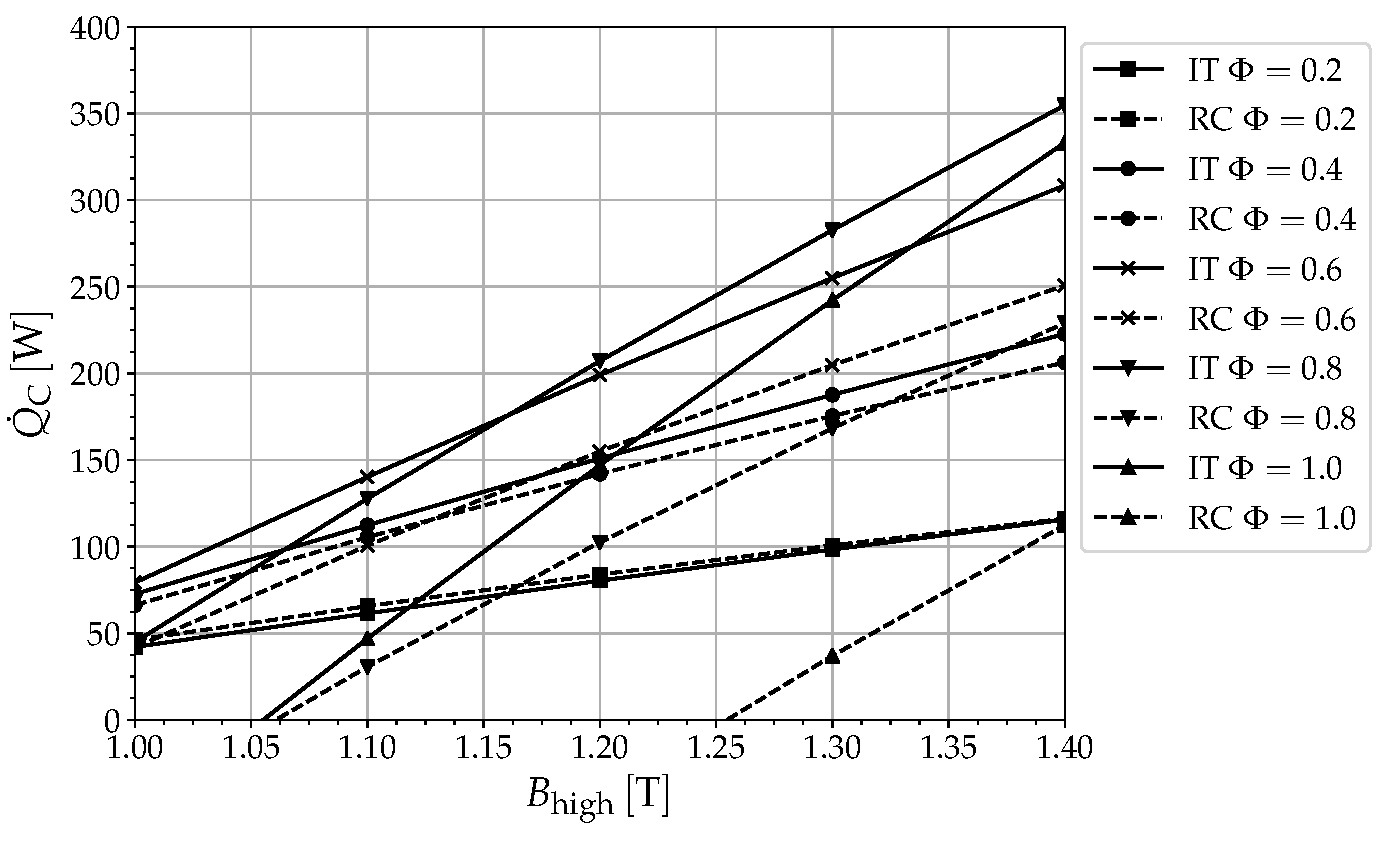
\includegraphics[width=8cm]{Qc_B_comp_f_1_same_minimum}\label{fig:comp_min}}
\,
%  \subfloat[Same average]{\includegraphics[width=8cm]{Qc_B_comp_f_1_same_low_average}\label{fig:comp_avg}}
\,
  \caption{Cooling capacity as a function of the  average high magnetic field, for different utilizations. “I”: instantaneous (blow fraction of \SI{100}{\percent}); “RC”: rectified cosine  (blow fraction of \SI{60}{\percent}), for both comparison methods.}
 \label{fig:cos_ins}
\end{figure}

The only exception in the ``same minimum'' comparison is seen for the lowest utilization of $\Phi = 0.2$, where the performance is slightly better for the RC profile. Since the blow fraction for the cosine is lower, the mass flow rate must be higher to yield the same utilization (cf. Eq.~\eqref{eq:2}), and this increases heat transfer rate, as previously explained ---  outweighing the effects of the magnetic field.

In general, the performance of the AMRs operating with the instantaneous magnetic profile yields better results. As can be seen on Fig.~\ref{fig:cos_ins}, an instantaneous profile with the lowest possible value of $\bmin$ and the highest possible value of $\bmax$, with a flow profile occupying the whole cycle with average values of utilization, results in the highest values of cooling capacity among all simulations, therefore, representing the ideal magnetic profile for an AMR.

\subsection{Analysis of the instantaneous profile}
\label{sec:deta-analys-inst}

As shown in the previous section, the instantaneous profile yields the highest values for cooling capacity. Therefore, in this section, a more detailed analysis of such profile has been carried out. Figure~\ref{fig:qc_phi_inst} shows the cooling capacity as function of utilization, for several levels of the maximum magnetic field for the instantaneous profile, for two different operating frequencies. Because of the conflicts between a low heat transfer rate for flow rates too low and a loss in regenerator effectiveness in flow rates too high, there are critical values of utilization that maximize cooling capacity, and this critical value grows with the level of magnetic field. With higher magnetic field, the increase in the MCE surpasses the loss of effectiveness, and one can go to higher flow rates without losing performance. It can also be seen in Fig.~\ref{fig:qc_phi_inst} that at higher frequencies, the values of cooling power are higher, and also the critical values of utilization are lower; however, this usually is achieved at the cost of higher power consumption in AMR devices at higher frequencies \cite{bib:lei15_study,NIKNIA2016601}.

\begin{figure}[!ht]
  \centering
\subfloat[$f = \SI{1}{\hertz}$]{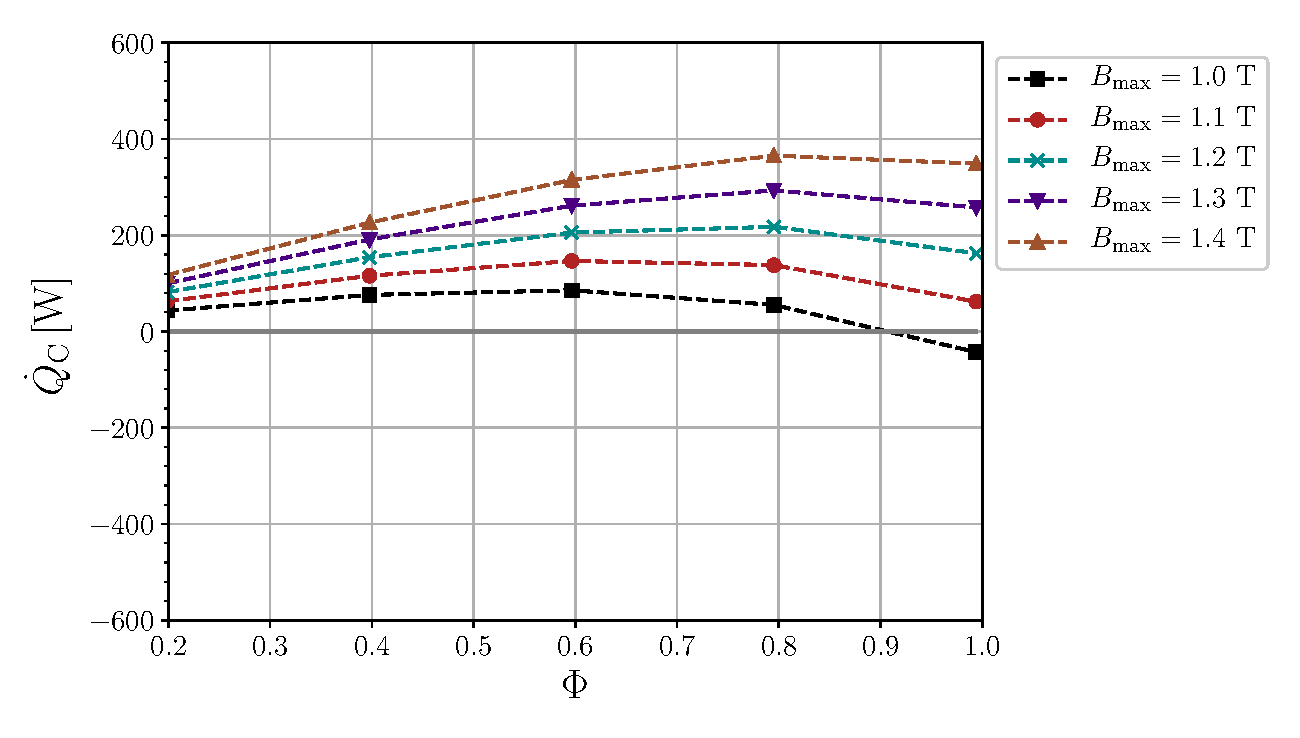
\includegraphics[width=8cm]{Qc_Phi_inst_f_1_Hmin_005_FB_100}\label{fig:Qc_phi_inst_1}}
\,
  \subfloat[$f = \SI{2}{\hertz}$]{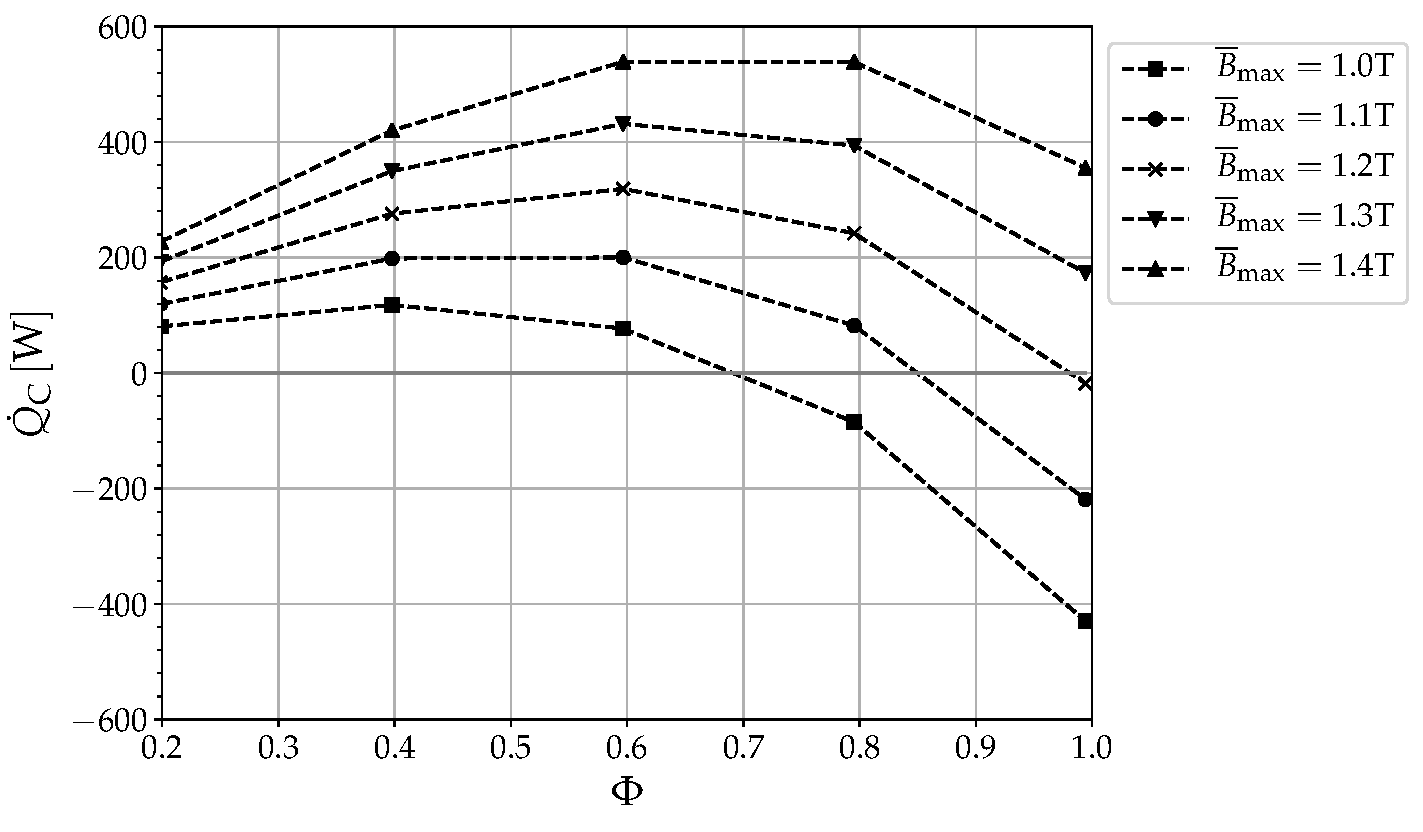
\includegraphics[width=8cm]{Qc_Phi_inst_f_2_Hmin_005_FB_100}\label{fig:Qc_phi_inst_2}}
  \caption{Cooling capacity as a function of utilization, for various values of the high magnetic field  of the instantaneous profile}
  \label{fig:qc_phi_inst}
\end{figure}

\begin{figure}[!ht]
  \centering
  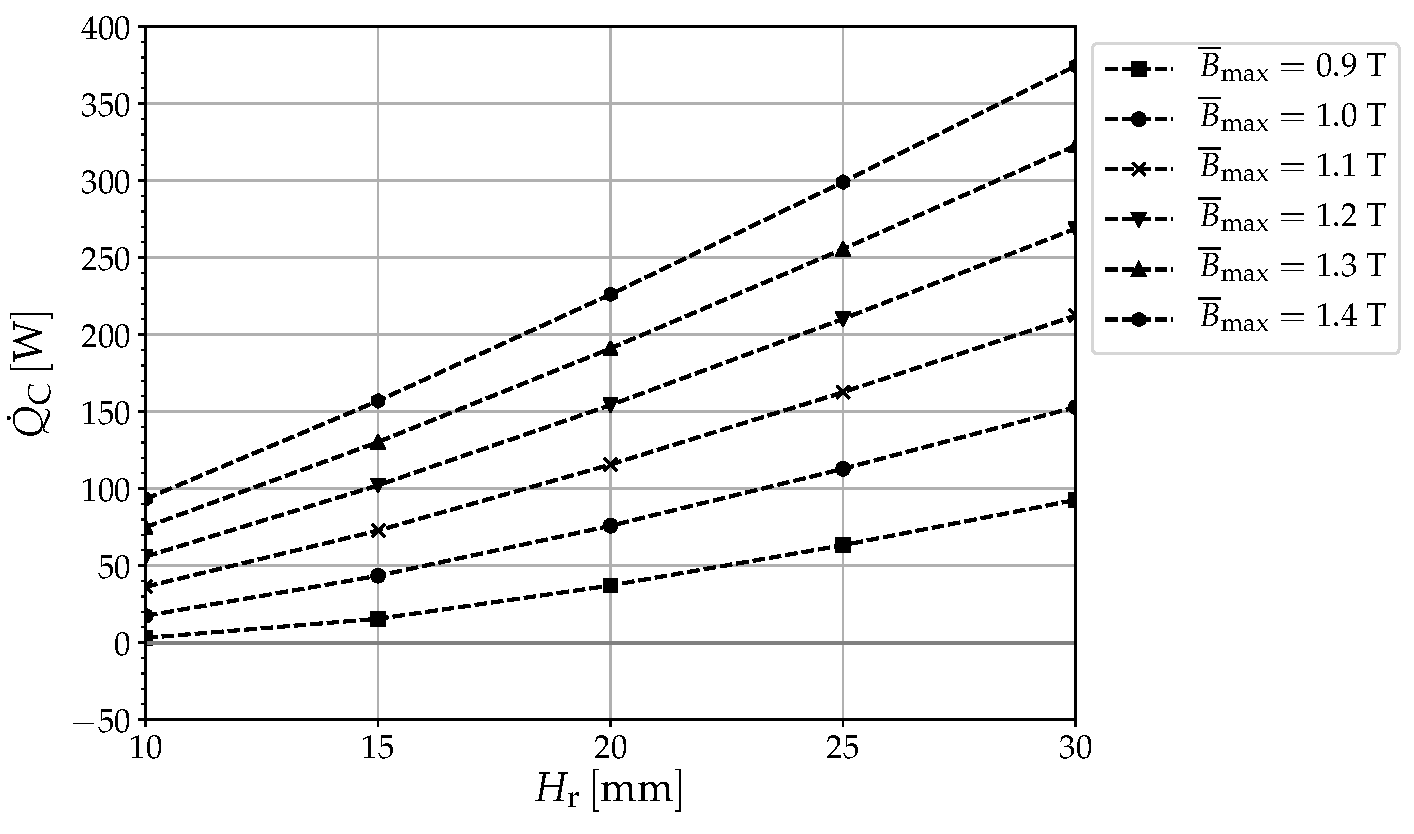
\includegraphics[width=8cm]{Qc_H_inst_f_1_Phi_40}
  \caption{Cooling capacity as a function of  regenerator height (all other parameters from Table~\ref{tab:params} constant) for various values of the high magnetic field of the instantaneous profile}
\label{fig:Qc_H_inst}
\end{figure}

The parameters in Table~\ref{tab:params} were chosen from preliminary simulations, but they are not guaranteed to be the optimal choices. To understand the impact of regenerator geometry on the performance with the instantaneous profile, the regenerator height was varied in Fig.~\ref{fig:Qc_H_inst}, and all other parameters from Table.~\ref{tab:params} were kept fixed. As expected, higher magnetic fields allow for smaller regenerators (and hence more compact systems). For instance, to achieve a capacity of \SI{100}{\watt}, increasing the field from \num{1.0} to \SI{1.2}{\tesla} result in using regenerators \SI{36}{\percent} smaller.

\section{CONCLUSIONS}
\label{sec:conclusions}

A one-dimensional AMR numerical model was used to compare the performance of a magnetic refrigerator under different operating and geometric parameters and with the instantaneous and rectified cosine magnetic profiles. Most of the AMRs operating with an instantaneous magnetic profile have resulted in better performances than those with a cosine profile, except in cases of low utilization. Although the cosine profile reaches higher levels of the magnetic field, the instantaneous profile can keep the magnetization (and demagnetization) for a longer period, which is shown to be beneficial to performance. Further analysis of the instantaneous profile has shown that the use of the highest possible value of the maximum magnetic field allows for using smaller regenerators and lower utilization, without losing performance.

\begin{acknowledgements}
This work was supported by CNPq, Embraco and EMBRAPII Unit Polo/UFSC.  
\end{acknowledgements}

% BibTeX users please use one of
%\bibliographystyle{spbasic}      % basic style, author-year citations
%\bibliographystyle{spmpsci}      % mathematics and physical sciences
\bibliographystyle{spphys}       % APS-like style for physics

\bibliography{thermo-ref/Thermo-Foam-Ref,thermo-ref/thesis}

\end{document}

%%% Local Variables:
%%% mode: latex
%%% TeX-master: t
%%% End:
